\documentclass[twoside]{book}

% Packages required by doxygen
\usepackage{fixltx2e}
\usepackage{calc}
\usepackage{doxygen}
\usepackage[export]{adjustbox} % also loads graphicx
\usepackage{graphicx}
\usepackage[utf8]{inputenc}
\usepackage{makeidx}
\usepackage{multicol}
\usepackage{multirow}
\PassOptionsToPackage{warn}{textcomp}
\usepackage{textcomp}
\usepackage[nointegrals]{wasysym}
\usepackage[table]{xcolor}

% Font selection
\usepackage[T1]{fontenc}
\usepackage[scaled=.90]{helvet}
\usepackage{courier}
\usepackage{amssymb}
\usepackage{sectsty}
\renewcommand{\familydefault}{\sfdefault}
\allsectionsfont{%
  \fontseries{bc}\selectfont%
  \color{darkgray}%
}
\renewcommand{\DoxyLabelFont}{%
  \fontseries{bc}\selectfont%
  \color{darkgray}%
}
\newcommand{\+}{\discretionary{\mbox{\scriptsize$\hookleftarrow$}}{}{}}

% Page & text layout
\usepackage{geometry}
\geometry{%
  a4paper,%
  top=2.5cm,%
  bottom=2.5cm,%
  left=2.5cm,%
  right=2.5cm%
}
\tolerance=750
\hfuzz=15pt
\hbadness=750
\setlength{\emergencystretch}{15pt}
\setlength{\parindent}{0cm}
\setlength{\parskip}{3ex plus 2ex minus 2ex}
\makeatletter
\renewcommand{\paragraph}{%
  \@startsection{paragraph}{4}{0ex}{-1.0ex}{1.0ex}{%
    \normalfont\normalsize\bfseries\SS@parafont%
  }%
}
\renewcommand{\subparagraph}{%
  \@startsection{subparagraph}{5}{0ex}{-1.0ex}{1.0ex}{%
    \normalfont\normalsize\bfseries\SS@subparafont%
  }%
}
\makeatother

% Headers & footers
\usepackage{fancyhdr}
\pagestyle{fancyplain}
\fancyhead[LE]{\fancyplain{}{\bfseries\thepage}}
\fancyhead[CE]{\fancyplain{}{}}
\fancyhead[RE]{\fancyplain{}{\bfseries\leftmark}}
\fancyhead[LO]{\fancyplain{}{\bfseries\rightmark}}
\fancyhead[CO]{\fancyplain{}{}}
\fancyhead[RO]{\fancyplain{}{\bfseries\thepage}}
\fancyfoot[LE]{\fancyplain{}{}}
\fancyfoot[CE]{\fancyplain{}{}}
\fancyfoot[RE]{\fancyplain{}{\bfseries\scriptsize Generated by Doxygen }}
\fancyfoot[LO]{\fancyplain{}{\bfseries\scriptsize Generated by Doxygen }}
\fancyfoot[CO]{\fancyplain{}{}}
\fancyfoot[RO]{\fancyplain{}{}}
\renewcommand{\footrulewidth}{0.4pt}
\renewcommand{\chaptermark}[1]{%
  \markboth{#1}{}%
}
\renewcommand{\sectionmark}[1]{%
  \markright{\thesection\ #1}%
}

% Indices & bibliography
\usepackage{natbib}
\usepackage[titles]{tocloft}
\setcounter{tocdepth}{3}
\setcounter{secnumdepth}{5}
\makeindex

% Hyperlinks (required, but should be loaded last)
\usepackage{ifpdf}
\ifpdf
  \usepackage[pdftex,pagebackref=true]{hyperref}
\else
  \usepackage[ps2pdf,pagebackref=true]{hyperref}
\fi
\hypersetup{%
  colorlinks=true,%
  linkcolor=blue,%
  citecolor=blue,%
  unicode%
}

% Custom commands
\newcommand{\clearemptydoublepage}{%
  \newpage{\pagestyle{empty}\cleardoublepage}%
}

\usepackage{caption}
\captionsetup{labelsep=space,justification=centering,font={bf},singlelinecheck=off,skip=4pt,position=top}

%===== C O N T E N T S =====

\begin{document}

% Titlepage & ToC
\hypersetup{pageanchor=false,
             bookmarksnumbered=true,
             pdfencoding=unicode
            }
\pagenumbering{alph}
\begin{titlepage}
\vspace*{7cm}
\begin{center}%
{\Large My Project \\[1ex]\large 1 }\\
\vspace*{1cm}
{\large Generated by Doxygen 1.8.13}\\
\end{center}
\end{titlepage}
\clearemptydoublepage
\pagenumbering{roman}
\tableofcontents
\clearemptydoublepage
\pagenumbering{arabic}
\hypersetup{pageanchor=true}

%--- Begin generated contents ---
\chapter{Class Index}
\section{Class List}
Here are the classes, structs, unions and interfaces with brief descriptions\+:\begin{DoxyCompactList}
\item\contentsline{section}{\hyperlink{struct_node}{Node} }{\pageref{struct_node}}{}
\end{DoxyCompactList}

\chapter{File Index}
\section{File List}
Here is a list of all files with brief descriptions\+:\begin{DoxyCompactList}
\item\contentsline{section}{Code/\hyperlink{tut6__q3_8cpp}{tut6\+\_\+q3.\+cpp} \\*This program implements Bentley-\/\+Ottmann Algorithm to find all intersection of n given lines and also find linear fit }{\pageref{tut6__q3_8cpp}}{}
\end{DoxyCompactList}

\chapter{Class Documentation}
\hypertarget{structadjl}{}\section{adjl Struct Reference}
\label{structadjl}\index{adjl@{adjl}}


structure to represent a list in adjacency list  




Collaboration diagram for adjl\+:
\nopagebreak
\begin{figure}[H]
\begin{center}
\leavevmode
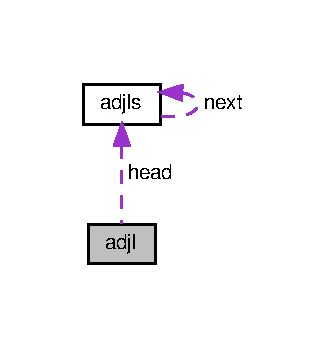
\includegraphics[width=157pt]{structadjl__coll__graph}
\end{center}
\end{figure}
\subsection*{Public Attributes}
\begin{DoxyCompactItemize}
\item 
\hyperlink{structadjls}{adjls} $\ast$ \hyperlink{structadjl_abb2ac2f6001871d6dbe505a55ce0277b}{head}
\end{DoxyCompactItemize}


\subsection{Detailed Description}
structure to represent a list in adjacency list 

Definition at line 20 of file main.\+cpp.



\subsection{Member Data Documentation}
\mbox{\Hypertarget{structadjl_abb2ac2f6001871d6dbe505a55ce0277b}\label{structadjl_abb2ac2f6001871d6dbe505a55ce0277b}} 
\index{adjl@{adjl}!head@{head}}
\index{head@{head}!adjl@{adjl}}
\subsubsection{\texorpdfstring{head}{head}}
{\footnotesize\ttfamily \hyperlink{structadjls}{adjls}$\ast$ adjl\+::head}



Definition at line 21 of file main.\+cpp.



The documentation for this struct was generated from the following file\+:\begin{DoxyCompactItemize}
\item 
Code/\hyperlink{main_8cpp}{main.\+cpp}\end{DoxyCompactItemize}

\hypertarget{structadjls}{}\section{adjls Struct Reference}
\label{structadjls}\index{adjls@{adjls}}


structure to represent each node in adjacency list  




Collaboration diagram for adjls\+:
\nopagebreak
\begin{figure}[H]
\begin{center}
\leavevmode
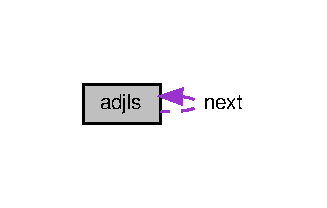
\includegraphics[width=157pt]{structadjls__coll__graph}
\end{center}
\end{figure}
\subsection*{Public Attributes}
\begin{DoxyCompactItemize}
\item 
int \hyperlink{structadjls_af69a07e0b1db5778735317a9b50f9caf}{data}
\item 
int \hyperlink{structadjls_a5436743f742db03491ad4b1a0e5a49a8}{distc}
\item 
int \hyperlink{structadjls_a9926ef0452fbfe40ec2d12ab41cf7e54}{dia}
\item 
\hyperlink{structadjls}{adjls} $\ast$ \hyperlink{structadjls_a5887ecb5fe66ccfbbb6748b6cd411259}{next}
\end{DoxyCompactItemize}


\subsection{Detailed Description}
structure to represent each node in adjacency list 

Definition at line 12 of file main.\+cpp.



\subsection{Member Data Documentation}
\mbox{\Hypertarget{structadjls_af69a07e0b1db5778735317a9b50f9caf}\label{structadjls_af69a07e0b1db5778735317a9b50f9caf}} 
\index{adjls@{adjls}!data@{data}}
\index{data@{data}!adjls@{adjls}}
\subsubsection{\texorpdfstring{data}{data}}
{\footnotesize\ttfamily int adjls\+::data}



Definition at line 13 of file main.\+cpp.

\mbox{\Hypertarget{structadjls_a9926ef0452fbfe40ec2d12ab41cf7e54}\label{structadjls_a9926ef0452fbfe40ec2d12ab41cf7e54}} 
\index{adjls@{adjls}!dia@{dia}}
\index{dia@{dia}!adjls@{adjls}}
\subsubsection{\texorpdfstring{dia}{dia}}
{\footnotesize\ttfamily int adjls\+::dia}



Definition at line 15 of file main.\+cpp.

\mbox{\Hypertarget{structadjls_a5436743f742db03491ad4b1a0e5a49a8}\label{structadjls_a5436743f742db03491ad4b1a0e5a49a8}} 
\index{adjls@{adjls}!distc@{distc}}
\index{distc@{distc}!adjls@{adjls}}
\subsubsection{\texorpdfstring{distc}{distc}}
{\footnotesize\ttfamily int adjls\+::distc}



Definition at line 14 of file main.\+cpp.

\mbox{\Hypertarget{structadjls_a5887ecb5fe66ccfbbb6748b6cd411259}\label{structadjls_a5887ecb5fe66ccfbbb6748b6cd411259}} 
\index{adjls@{adjls}!next@{next}}
\index{next@{next}!adjls@{adjls}}
\subsubsection{\texorpdfstring{next}{next}}
{\footnotesize\ttfamily \hyperlink{structadjls}{adjls}$\ast$ adjls\+::next}



Definition at line 16 of file main.\+cpp.



The documentation for this struct was generated from the following file\+:\begin{DoxyCompactItemize}
\item 
Code/\hyperlink{main_8cpp}{main.\+cpp}\end{DoxyCompactItemize}

\hypertarget{struct_graph}{}\section{Graph Struct Reference}
\label{struct_graph}\index{Graph@{Graph}}
\subsection*{Public Member Functions}
\begin{DoxyCompactItemize}
\item 
\hyperlink{struct_graph_ad3b98f95ee53f91afad11b8eaddc35e0}{Graph} (int \hyperlink{struct_graph_a2b722f7cfa7a21e4cb5fae488b3d4dcc}{V}, int \hyperlink{struct_graph_a3ce250f958f7e96ffd9eb06780c21fbe}{E})
\item 
void \hyperlink{struct_graph_ab7b4b061fdba1d19a5fbcee110a319bd}{add\+Edge} (int u, int v, int w)
\item 
int \hyperlink{struct_graph_acec80ad3aef831280f7a05217270fb7b}{kruskal\+M\+ST} ()
\end{DoxyCompactItemize}
\subsection*{Public Attributes}
\begin{DoxyCompactItemize}
\item 
int \hyperlink{struct_graph_a2b722f7cfa7a21e4cb5fae488b3d4dcc}{V}
\item 
int \hyperlink{struct_graph_a3ce250f958f7e96ffd9eb06780c21fbe}{E}
\item 
vector$<$ pair$<$ int, \hyperlink{q22_8cpp_a18fc5862b3095bd9855a9e15c67b392d}{i\+Pair} $>$ $>$ \hyperlink{struct_graph_a6694959510dc3092c7a02efa56ed7a8f}{edges}
\end{DoxyCompactItemize}


\subsection{Detailed Description}


Definition at line 14 of file q22.\+cpp.



\subsection{Constructor \& Destructor Documentation}
\mbox{\Hypertarget{struct_graph_ad3b98f95ee53f91afad11b8eaddc35e0}\label{struct_graph_ad3b98f95ee53f91afad11b8eaddc35e0}} 
\index{Graph@{Graph}!Graph@{Graph}}
\index{Graph@{Graph}!Graph@{Graph}}
\subsubsection{\texorpdfstring{Graph()}{Graph()}}
{\footnotesize\ttfamily Graph\+::\+Graph (\begin{DoxyParamCaption}\item[{int}]{V,  }\item[{int}]{E }\end{DoxyParamCaption})\hspace{0.3cm}{\ttfamily [inline]}}



Definition at line 20 of file q22.\+cpp.



\subsection{Member Function Documentation}
\mbox{\Hypertarget{struct_graph_ab7b4b061fdba1d19a5fbcee110a319bd}\label{struct_graph_ab7b4b061fdba1d19a5fbcee110a319bd}} 
\index{Graph@{Graph}!add\+Edge@{add\+Edge}}
\index{add\+Edge@{add\+Edge}!Graph@{Graph}}
\subsubsection{\texorpdfstring{add\+Edge()}{addEdge()}}
{\footnotesize\ttfamily void Graph\+::add\+Edge (\begin{DoxyParamCaption}\item[{int}]{u,  }\item[{int}]{v,  }\item[{int}]{w }\end{DoxyParamCaption})\hspace{0.3cm}{\ttfamily [inline]}}



Definition at line 27 of file q22.\+cpp.

\mbox{\Hypertarget{struct_graph_acec80ad3aef831280f7a05217270fb7b}\label{struct_graph_acec80ad3aef831280f7a05217270fb7b}} 
\index{Graph@{Graph}!kruskal\+M\+ST@{kruskal\+M\+ST}}
\index{kruskal\+M\+ST@{kruskal\+M\+ST}!Graph@{Graph}}
\subsubsection{\texorpdfstring{kruskal\+M\+S\+T()}{kruskalMST()}}
{\footnotesize\ttfamily int Graph\+::kruskal\+M\+ST (\begin{DoxyParamCaption}{ }\end{DoxyParamCaption})}



Definition at line 92 of file q22.\+cpp.



\subsection{Member Data Documentation}
\mbox{\Hypertarget{struct_graph_a3ce250f958f7e96ffd9eb06780c21fbe}\label{struct_graph_a3ce250f958f7e96ffd9eb06780c21fbe}} 
\index{Graph@{Graph}!E@{E}}
\index{E@{E}!Graph@{Graph}}
\subsubsection{\texorpdfstring{E}{E}}
{\footnotesize\ttfamily int Graph\+::E}



Definition at line 16 of file q22.\+cpp.

\mbox{\Hypertarget{struct_graph_a6694959510dc3092c7a02efa56ed7a8f}\label{struct_graph_a6694959510dc3092c7a02efa56ed7a8f}} 
\index{Graph@{Graph}!edges@{edges}}
\index{edges@{edges}!Graph@{Graph}}
\subsubsection{\texorpdfstring{edges}{edges}}
{\footnotesize\ttfamily vector$<$ pair$<$int, \hyperlink{q22_8cpp_a18fc5862b3095bd9855a9e15c67b392d}{i\+Pair}$>$ $>$ Graph\+::edges}



Definition at line 17 of file q22.\+cpp.

\mbox{\Hypertarget{struct_graph_a2b722f7cfa7a21e4cb5fae488b3d4dcc}\label{struct_graph_a2b722f7cfa7a21e4cb5fae488b3d4dcc}} 
\index{Graph@{Graph}!V@{V}}
\index{V@{V}!Graph@{Graph}}
\subsubsection{\texorpdfstring{V}{V}}
{\footnotesize\ttfamily int Graph\+::V}



Definition at line 16 of file q22.\+cpp.



The documentation for this struct was generated from the following file\+:\begin{DoxyCompactItemize}
\item 
Code/\hyperlink{q22_8cpp}{q22.\+cpp}\end{DoxyCompactItemize}

\hypertarget{struct_node}{}\section{Node Struct Reference}
\label{struct_node}\index{Node@{Node}}
\subsection*{Public Attributes}
\begin{DoxyCompactItemize}
\item 
int \hyperlink{struct_node_a2fdf3febffa37539c09d0a282525033a}{a}
\item 
int \hyperlink{struct_node_a26cb9e26541900f36489bf503338ce4e}{b} \mbox{[}100\mbox{]}
\item 
int \hyperlink{struct_node_acc103d220defd2fdb5aac8e3b03424c6}{size} =0
\end{DoxyCompactItemize}


\subsection{Detailed Description}


Definition at line 8 of file Q1\+\_\+v2.\+cpp.



\subsection{Member Data Documentation}
\mbox{\Hypertarget{struct_node_a2fdf3febffa37539c09d0a282525033a}\label{struct_node_a2fdf3febffa37539c09d0a282525033a}} 
\index{Node@{Node}!a@{a}}
\index{a@{a}!Node@{Node}}
\subsubsection{\texorpdfstring{a}{a}}
{\footnotesize\ttfamily int Node\+::a}



Definition at line 9 of file Q1\+\_\+v2.\+cpp.

\mbox{\Hypertarget{struct_node_a26cb9e26541900f36489bf503338ce4e}\label{struct_node_a26cb9e26541900f36489bf503338ce4e}} 
\index{Node@{Node}!b@{b}}
\index{b@{b}!Node@{Node}}
\subsubsection{\texorpdfstring{b}{b}}
{\footnotesize\ttfamily int Node\+::b\mbox{[}100\mbox{]}}



Definition at line 10 of file Q1\+\_\+v2.\+cpp.

\mbox{\Hypertarget{struct_node_acc103d220defd2fdb5aac8e3b03424c6}\label{struct_node_acc103d220defd2fdb5aac8e3b03424c6}} 
\index{Node@{Node}!size@{size}}
\index{size@{size}!Node@{Node}}
\subsubsection{\texorpdfstring{size}{size}}
{\footnotesize\ttfamily int Node\+::size =0}



Definition at line 11 of file Q1\+\_\+v2.\+cpp.



The documentation for this struct was generated from the following file\+:\begin{DoxyCompactItemize}
\item 
Code/\hyperlink{_q1__v2_8cpp}{Q1\+\_\+v2.\+cpp}\end{DoxyCompactItemize}

\chapter{File Documentation}
\hypertarget{main_8cpp}{}\doxysection{C\+:/\+Users/\+Rushi/\+Desktop/\+Assignment\+\_\+3/\+P2/code/main.cpp File Reference}
\label{main_8cpp}\index{C:/Users/Rushi/Desktop/Assignment\_3/P2/code/main.cpp@{C:/Users/Rushi/Desktop/Assignment\_3/P2/code/main.cpp}}
{\ttfamily \#include $<$stdio.\+h$>$}\newline
{\ttfamily \#include $<$stdlib.\+h$>$}\newline
{\ttfamily \#include $<$string.\+h$>$}\newline
\doxysubsection*{Data Structures}
\begin{DoxyCompactItemize}
\item 
struct \mbox{\hyperlink{struct_que_node}{Que\+Node}}
\item 
struct \mbox{\hyperlink{struct_node}{Node}}
\end{DoxyCompactItemize}
\doxysubsection*{Functions}
\begin{DoxyCompactItemize}
\item 
void \mbox{\hyperlink{main_8cpp_a7cf73e85e61c143173cc765beae8ee4b}{store}} (int i2, int j2, int k2)
\item 
void \mbox{\hyperlink{main_8cpp_a55c3cc33aa878501ddb38eda82bbcbe8}{insert}} (int d)
\item 
int \mbox{\hyperlink{main_8cpp_ae14368f69c4359050a5d88cab50a5cdf}{Xorfunc}} (struct \mbox{\hyperlink{struct_node}{Node}} $\ast$head, struct \mbox{\hyperlink{struct_node}{Node}} $\ast$rear)
\item 
int \mbox{\hyperlink{main_8cpp_ad079eaa5d70a919fa497e5e3ab7c8dad}{count}} (struct \mbox{\hyperlink{struct_node}{Node}} $\ast$head, struct \mbox{\hyperlink{struct_node}{Node}} $\ast$rear, int i, int k)
\item 
int \mbox{\hyperlink{main_8cpp_a01dea55abcc3972c791244c0ee03cb8b}{count\+Triplets}} (struct \mbox{\hyperlink{struct_node}{Node}} $\ast$hd, struct \mbox{\hyperlink{struct_node}{Node}} $\ast$lst)
\item 
void \mbox{\hyperlink{main_8cpp_a4b05ced400ef492052a1d50e2755d71a}{show\+Triplets}} ()
\item 
int \mbox{\hyperlink{main_8cpp_ae66f6b31b5ad750f1fe042a706a4e3d4}{main}} ()
\end{DoxyCompactItemize}
\doxysubsection*{Variables}
\begin{DoxyCompactItemize}
\item 
struct \mbox{\hyperlink{struct_que_node}{Que\+Node}} $\ast$ \mbox{\hyperlink{main_8cpp_ac98657983f5f9710235d99c98ef56087}{Que\+First}} = N\+U\+LL
\item 
struct \mbox{\hyperlink{struct_que_node}{Que\+Node}} $\ast$ \mbox{\hyperlink{main_8cpp_af9a79b1b8e625db223ddfd617894af22}{Que\+Last}} =N\+U\+LL
\item 
struct \mbox{\hyperlink{struct_node}{Node}} $\ast$ \mbox{\hyperlink{main_8cpp_ad4f551b04c42cff59f7823e0ec1bc90e}{first}} = N\+U\+LL
\item 
struct \mbox{\hyperlink{struct_node}{Node}} $\ast$ \mbox{\hyperlink{main_8cpp_ad55f91e3773370b790704d512696ad6d}{last}} =N\+U\+LL
\item 
int \mbox{\hyperlink{main_8cpp_a9f59b34b1f25fe00023291b678246bcc}{length}} =0
\end{DoxyCompactItemize}


\doxysubsection{Function Documentation}
\mbox{\Hypertarget{main_8cpp_ad079eaa5d70a919fa497e5e3ab7c8dad}\label{main_8cpp_ad079eaa5d70a919fa497e5e3ab7c8dad}} 
\index{main.cpp@{main.cpp}!count@{count}}
\index{count@{count}!main.cpp@{main.cpp}}
\doxysubsubsection{\texorpdfstring{count()}{count()}}
{\footnotesize\ttfamily int count (\begin{DoxyParamCaption}\item[{struct \mbox{\hyperlink{struct_node}{Node}} $\ast$}]{head,  }\item[{struct \mbox{\hyperlink{struct_node}{Node}} $\ast$}]{rear,  }\item[{int}]{i,  }\item[{int}]{k }\end{DoxyParamCaption})}

This method counts the number of j. \begin{DoxyAuthor}{Author}
Rushiprasad 
\end{DoxyAuthor}

\begin{DoxyParams}{Parameters}
{\em Node$\ast$} & head start point \\
\hline
{\em Node$\ast$} & rear end point \\
\hline
{\em i} & changing start point \\
\hline
{\em j} & changing end point \\
\hline
\end{DoxyParams}
\begin{DoxyDate}{Date}
21/08/2019 
\end{DoxyDate}


Definition at line 113 of file main.\+cpp.

\mbox{\Hypertarget{main_8cpp_a01dea55abcc3972c791244c0ee03cb8b}\label{main_8cpp_a01dea55abcc3972c791244c0ee03cb8b}} 
\index{main.cpp@{main.cpp}!countTriplets@{countTriplets}}
\index{countTriplets@{countTriplets}!main.cpp@{main.cpp}}
\doxysubsubsection{\texorpdfstring{countTriplets()}{countTriplets()}}
{\footnotesize\ttfamily int count\+Triplets (\begin{DoxyParamCaption}\item[{struct \mbox{\hyperlink{struct_node}{Node}} $\ast$}]{hd,  }\item[{struct \mbox{\hyperlink{struct_node}{Node}} $\ast$}]{lst }\end{DoxyParamCaption})}

This method counts the number of triplets. \begin{DoxyAuthor}{Author}
Rushiprasad 
\end{DoxyAuthor}

\begin{DoxyParams}{Parameters}
{\em Node$\ast$} & hd start point \\
\hline
{\em Node$\ast$} & lst end point \\
\hline
\end{DoxyParams}
\begin{DoxyDate}{Date}
21/08/2019 
\end{DoxyDate}


Definition at line 137 of file main.\+cpp.

\mbox{\Hypertarget{main_8cpp_a55c3cc33aa878501ddb38eda82bbcbe8}\label{main_8cpp_a55c3cc33aa878501ddb38eda82bbcbe8}} 
\index{main.cpp@{main.cpp}!insert@{insert}}
\index{insert@{insert}!main.cpp@{main.cpp}}
\doxysubsubsection{\texorpdfstring{insert()}{insert()}}
{\footnotesize\ttfamily void insert (\begin{DoxyParamCaption}\item[{int}]{d }\end{DoxyParamCaption})}

This method will insert an element to linked list. \begin{DoxyAuthor}{Author}
Rushiprasad 
\end{DoxyAuthor}

\begin{DoxyParams}{Parameters}
{\em d} & key value to be inserted in linked list \\
\hline
\end{DoxyParams}
\begin{DoxyDate}{Date}
21/08/2019 
\end{DoxyDate}


Definition at line 69 of file main.\+cpp.

\mbox{\Hypertarget{main_8cpp_ae66f6b31b5ad750f1fe042a706a4e3d4}\label{main_8cpp_ae66f6b31b5ad750f1fe042a706a4e3d4}} 
\index{main.cpp@{main.cpp}!main@{main}}
\index{main@{main}!main.cpp@{main.cpp}}
\doxysubsubsection{\texorpdfstring{main()}{main()}}
{\footnotesize\ttfamily int main (\begin{DoxyParamCaption}{ }\end{DoxyParamCaption})}



Definition at line 173 of file main.\+cpp.

\mbox{\Hypertarget{main_8cpp_a4b05ced400ef492052a1d50e2755d71a}\label{main_8cpp_a4b05ced400ef492052a1d50e2755d71a}} 
\index{main.cpp@{main.cpp}!showTriplets@{showTriplets}}
\index{showTriplets@{showTriplets}!main.cpp@{main.cpp}}
\doxysubsubsection{\texorpdfstring{showTriplets()}{showTriplets()}}
{\footnotesize\ttfamily void show\+Triplets (\begin{DoxyParamCaption}{ }\end{DoxyParamCaption})}

This method prints the triplets. \begin{DoxyAuthor}{Author}
Rushiprasad 
\end{DoxyAuthor}
\begin{DoxyDate}{Date}
21/08/2019 
\end{DoxyDate}


Definition at line 165 of file main.\+cpp.

\mbox{\Hypertarget{main_8cpp_a7cf73e85e61c143173cc765beae8ee4b}\label{main_8cpp_a7cf73e85e61c143173cc765beae8ee4b}} 
\index{main.cpp@{main.cpp}!store@{store}}
\index{store@{store}!main.cpp@{main.cpp}}
\doxysubsubsection{\texorpdfstring{store()}{store()}}
{\footnotesize\ttfamily void store (\begin{DoxyParamCaption}\item[{int}]{i2,  }\item[{int}]{j2,  }\item[{int}]{k2 }\end{DoxyParamCaption})}



Definition at line 37 of file main.\+cpp.

\mbox{\Hypertarget{main_8cpp_ae14368f69c4359050a5d88cab50a5cdf}\label{main_8cpp_ae14368f69c4359050a5d88cab50a5cdf}} 
\index{main.cpp@{main.cpp}!Xorfunc@{Xorfunc}}
\index{Xorfunc@{Xorfunc}!main.cpp@{main.cpp}}
\doxysubsubsection{\texorpdfstring{Xorfunc()}{Xorfunc()}}
{\footnotesize\ttfamily int Xorfunc (\begin{DoxyParamCaption}\item[{struct \mbox{\hyperlink{struct_node}{Node}} $\ast$}]{head,  }\item[{struct \mbox{\hyperlink{struct_node}{Node}} $\ast$}]{rear }\end{DoxyParamCaption})}

This method xors the numbers between a range given. \begin{DoxyAuthor}{Author}
Rushiprasad 
\end{DoxyAuthor}

\begin{DoxyParams}{Parameters}
{\em Node$\ast$} & head start point \\
\hline
{\em Node$\ast$} & rear end point \\
\hline
\end{DoxyParams}
\begin{DoxyDate}{Date}
21/08/2019 
\end{DoxyDate}


Definition at line 94 of file main.\+cpp.



\doxysubsection{Variable Documentation}
\mbox{\Hypertarget{main_8cpp_ad4f551b04c42cff59f7823e0ec1bc90e}\label{main_8cpp_ad4f551b04c42cff59f7823e0ec1bc90e}} 
\index{main.cpp@{main.cpp}!first@{first}}
\index{first@{first}!main.cpp@{main.cpp}}
\doxysubsubsection{\texorpdfstring{first}{first}}
{\footnotesize\ttfamily struct \mbox{\hyperlink{struct_node}{Node}}$\ast$ first = N\+U\+LL}



Definition at line 59 of file main.\+cpp.

\mbox{\Hypertarget{main_8cpp_ad55f91e3773370b790704d512696ad6d}\label{main_8cpp_ad55f91e3773370b790704d512696ad6d}} 
\index{main.cpp@{main.cpp}!last@{last}}
\index{last@{last}!main.cpp@{main.cpp}}
\doxysubsubsection{\texorpdfstring{last}{last}}
{\footnotesize\ttfamily struct \mbox{\hyperlink{struct_node}{Node}} $\ast$ last =N\+U\+LL}



Definition at line 59 of file main.\+cpp.

\mbox{\Hypertarget{main_8cpp_a9f59b34b1f25fe00023291b678246bcc}\label{main_8cpp_a9f59b34b1f25fe00023291b678246bcc}} 
\index{main.cpp@{main.cpp}!length@{length}}
\index{length@{length}!main.cpp@{main.cpp}}
\doxysubsubsection{\texorpdfstring{length}{length}}
{\footnotesize\ttfamily int length =0}



Definition at line 60 of file main.\+cpp.

\mbox{\Hypertarget{main_8cpp_ac98657983f5f9710235d99c98ef56087}\label{main_8cpp_ac98657983f5f9710235d99c98ef56087}} 
\index{main.cpp@{main.cpp}!QueFirst@{QueFirst}}
\index{QueFirst@{QueFirst}!main.cpp@{main.cpp}}
\doxysubsubsection{\texorpdfstring{QueFirst}{QueFirst}}
{\footnotesize\ttfamily struct \mbox{\hyperlink{struct_que_node}{Que\+Node}}$\ast$ Que\+First = N\+U\+LL}



Definition at line 36 of file main.\+cpp.

\mbox{\Hypertarget{main_8cpp_af9a79b1b8e625db223ddfd617894af22}\label{main_8cpp_af9a79b1b8e625db223ddfd617894af22}} 
\index{main.cpp@{main.cpp}!QueLast@{QueLast}}
\index{QueLast@{QueLast}!main.cpp@{main.cpp}}
\doxysubsubsection{\texorpdfstring{QueLast}{QueLast}}
{\footnotesize\ttfamily struct \mbox{\hyperlink{struct_que_node}{Que\+Node}} $\ast$ Que\+Last =N\+U\+LL}



Definition at line 36 of file main.\+cpp.


\hypertarget{_q1__v2_8cpp}{}\section{Code/\+Q1\+\_\+v2.cpp File Reference}
\label{_q1__v2_8cpp}\index{Code/\+Q1\+\_\+v2.\+cpp@{Code/\+Q1\+\_\+v2.\+cpp}}
{\ttfamily \#include $<$bits/stdc++.\+h$>$}\newline
Include dependency graph for Q1\+\_\+v2.\+cpp\+:
\nopagebreak
\begin{figure}[H]
\begin{center}
\leavevmode
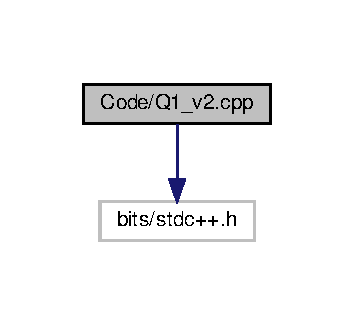
\includegraphics[width=170pt]{_q1__v2_8cpp__incl}
\end{center}
\end{figure}
\subsection*{Classes}
\begin{DoxyCompactItemize}
\item 
struct \hyperlink{struct_node}{Node}
\end{DoxyCompactItemize}
\subsection*{Typedefs}
\begin{DoxyCompactItemize}
\item 
typedef long long int \hyperlink{_q1__v2_8cpp_a1ae942ac54ad537f51a8f7d3723f61d7}{ll}
\end{DoxyCompactItemize}
\subsection*{Functions}
\begin{DoxyCompactItemize}
\item 
void \hyperlink{_q1__v2_8cpp_afe131eff8926689d02c0003e42daca61}{depth\+\_\+first\+\_\+search} (\hyperlink{struct_node}{Node} graph\mbox{[}$\,$\mbox{]}, bool visited\mbox{[}$\,$\mbox{]}, int current)
\item 
void \hyperlink{_q1__v2_8cpp_a5ed3b1a37d2da3a9f90e19ca5c939fee}{bredth\+\_\+first\+\_\+search} (\hyperlink{struct_node}{Node} graph\mbox{[}$\,$\mbox{]}, bool visited\mbox{[}$\,$\mbox{]})
\item 
bool \hyperlink{_q1__v2_8cpp_a6252ebbf4cdb8d5796e894e1418f5578}{cycle} (\hyperlink{struct_node}{Node} graph\mbox{[}$\,$\mbox{]})
\item 
void \hyperlink{_q1__v2_8cpp_a51ea66693faa73fc6eb8e595ed4c8023}{diadepth\+\_\+first\+\_\+search} (\hyperlink{struct_node}{Node} graph\mbox{[}$\,$\mbox{]}, int current, int dis\mbox{[}100\mbox{]}, int d)
\item 
int \hyperlink{_q1__v2_8cpp_ae66f6b31b5ad750f1fe042a706a4e3d4}{main} ()
\end{DoxyCompactItemize}


\subsection{Typedef Documentation}
\mbox{\Hypertarget{_q1__v2_8cpp_a1ae942ac54ad537f51a8f7d3723f61d7}\label{_q1__v2_8cpp_a1ae942ac54ad537f51a8f7d3723f61d7}} 
\index{Q1\+\_\+v2.\+cpp@{Q1\+\_\+v2.\+cpp}!ll@{ll}}
\index{ll@{ll}!Q1\+\_\+v2.\+cpp@{Q1\+\_\+v2.\+cpp}}
\subsubsection{\texorpdfstring{ll}{ll}}
{\footnotesize\ttfamily typedef long long int \hyperlink{_q1__v2_8cpp_a1ae942ac54ad537f51a8f7d3723f61d7}{ll}}



Definition at line 6 of file Q1\+\_\+v2.\+cpp.



\subsection{Function Documentation}
\mbox{\Hypertarget{_q1__v2_8cpp_a5ed3b1a37d2da3a9f90e19ca5c939fee}\label{_q1__v2_8cpp_a5ed3b1a37d2da3a9f90e19ca5c939fee}} 
\index{Q1\+\_\+v2.\+cpp@{Q1\+\_\+v2.\+cpp}!bredth\+\_\+first\+\_\+search@{bredth\+\_\+first\+\_\+search}}
\index{bredth\+\_\+first\+\_\+search@{bredth\+\_\+first\+\_\+search}!Q1\+\_\+v2.\+cpp@{Q1\+\_\+v2.\+cpp}}
\subsubsection{\texorpdfstring{bredth\+\_\+first\+\_\+search()}{bredth\_first\_search()}}
{\footnotesize\ttfamily void bredth\+\_\+first\+\_\+search (\begin{DoxyParamCaption}\item[{\hyperlink{struct_node}{Node}}]{graph\mbox{[}$\,$\mbox{]},  }\item[{bool}]{visited\mbox{[}$\,$\mbox{]} }\end{DoxyParamCaption})}



Definition at line 26 of file Q1\+\_\+v2.\+cpp.

\mbox{\Hypertarget{_q1__v2_8cpp_a6252ebbf4cdb8d5796e894e1418f5578}\label{_q1__v2_8cpp_a6252ebbf4cdb8d5796e894e1418f5578}} 
\index{Q1\+\_\+v2.\+cpp@{Q1\+\_\+v2.\+cpp}!cycle@{cycle}}
\index{cycle@{cycle}!Q1\+\_\+v2.\+cpp@{Q1\+\_\+v2.\+cpp}}
\subsubsection{\texorpdfstring{cycle()}{cycle()}}
{\footnotesize\ttfamily bool cycle (\begin{DoxyParamCaption}\item[{\hyperlink{struct_node}{Node}}]{graph\mbox{[}$\,$\mbox{]} }\end{DoxyParamCaption})}



Definition at line 45 of file Q1\+\_\+v2.\+cpp.

\mbox{\Hypertarget{_q1__v2_8cpp_afe131eff8926689d02c0003e42daca61}\label{_q1__v2_8cpp_afe131eff8926689d02c0003e42daca61}} 
\index{Q1\+\_\+v2.\+cpp@{Q1\+\_\+v2.\+cpp}!depth\+\_\+first\+\_\+search@{depth\+\_\+first\+\_\+search}}
\index{depth\+\_\+first\+\_\+search@{depth\+\_\+first\+\_\+search}!Q1\+\_\+v2.\+cpp@{Q1\+\_\+v2.\+cpp}}
\subsubsection{\texorpdfstring{depth\+\_\+first\+\_\+search()}{depth\_first\_search()}}
{\footnotesize\ttfamily void depth\+\_\+first\+\_\+search (\begin{DoxyParamCaption}\item[{\hyperlink{struct_node}{Node}}]{graph\mbox{[}$\,$\mbox{]},  }\item[{bool}]{visited\mbox{[}$\,$\mbox{]},  }\item[{int}]{current }\end{DoxyParamCaption})}



Definition at line 13 of file Q1\+\_\+v2.\+cpp.

\mbox{\Hypertarget{_q1__v2_8cpp_a51ea66693faa73fc6eb8e595ed4c8023}\label{_q1__v2_8cpp_a51ea66693faa73fc6eb8e595ed4c8023}} 
\index{Q1\+\_\+v2.\+cpp@{Q1\+\_\+v2.\+cpp}!diadepth\+\_\+first\+\_\+search@{diadepth\+\_\+first\+\_\+search}}
\index{diadepth\+\_\+first\+\_\+search@{diadepth\+\_\+first\+\_\+search}!Q1\+\_\+v2.\+cpp@{Q1\+\_\+v2.\+cpp}}
\subsubsection{\texorpdfstring{diadepth\+\_\+first\+\_\+search()}{diadepth\_first\_search()}}
{\footnotesize\ttfamily void diadepth\+\_\+first\+\_\+search (\begin{DoxyParamCaption}\item[{\hyperlink{struct_node}{Node}}]{graph\mbox{[}$\,$\mbox{]},  }\item[{int}]{current,  }\item[{int}]{dis\mbox{[}100\mbox{]},  }\item[{int}]{d }\end{DoxyParamCaption})}



Definition at line 60 of file Q1\+\_\+v2.\+cpp.

\mbox{\Hypertarget{_q1__v2_8cpp_ae66f6b31b5ad750f1fe042a706a4e3d4}\label{_q1__v2_8cpp_ae66f6b31b5ad750f1fe042a706a4e3d4}} 
\index{Q1\+\_\+v2.\+cpp@{Q1\+\_\+v2.\+cpp}!main@{main}}
\index{main@{main}!Q1\+\_\+v2.\+cpp@{Q1\+\_\+v2.\+cpp}}
\subsubsection{\texorpdfstring{main()}{main()}}
{\footnotesize\ttfamily int main (\begin{DoxyParamCaption}{ }\end{DoxyParamCaption})}



Definition at line 71 of file Q1\+\_\+v2.\+cpp.


%--- End generated contents ---

% Index
\backmatter
\newpage
\phantomsection
\clearemptydoublepage
\addcontentsline{toc}{chapter}{Index}
\printindex

\end{document}
